% Teilauswertung X

\section{Empfindlichkeit der FM-Apparatur und Konversionsverluste des Mischers}
\label{sec:verlusteAuswertung}

\subsection{Vergleich der Spektrumanalysatorwerte}
\label{sub:specAnalVergleich}

Zuerst wird die Theorie mit der Praxis verglichen. Dafür werden die Werte dem Spektrumanalysator mit den gemessenen Werten aus Kapitel \ref{sub:verluste} [Tab. \ref{tab:specAnal}] zu den theoretischen Werten aus Kapitel \ref{sec:signalAbsorp} in Kontrast gesetzt. Dafür wird für $P_\mathrm{S,Theo} = -22$\,dBm und für $P_\mathrm{R,Theo}= -77$\,dBm ($P_\mathrm{R,Theo} = P_\mathrm{S,Theo} - 55\,\mathrm{dB}$), wobei die 55\,dB die Leistungsverstärkung des HF-Verstärkers ist. In Abbildung \ref{fig:specAnalVergleich} lässt sich erkennen, im Bereich der gemessenen Werte liegen nur vereinzelt bei niedrigen Frequenzen für die Modulationsfrequenz $\omega_\mathrm{m}$ leicht niedrigere Werte, was aber gut mit dem Ablesefehler der Werte vom Spektrumanalysator zusammenhängen kann.
\begin{center}
    \captionsetup{type=figure}
    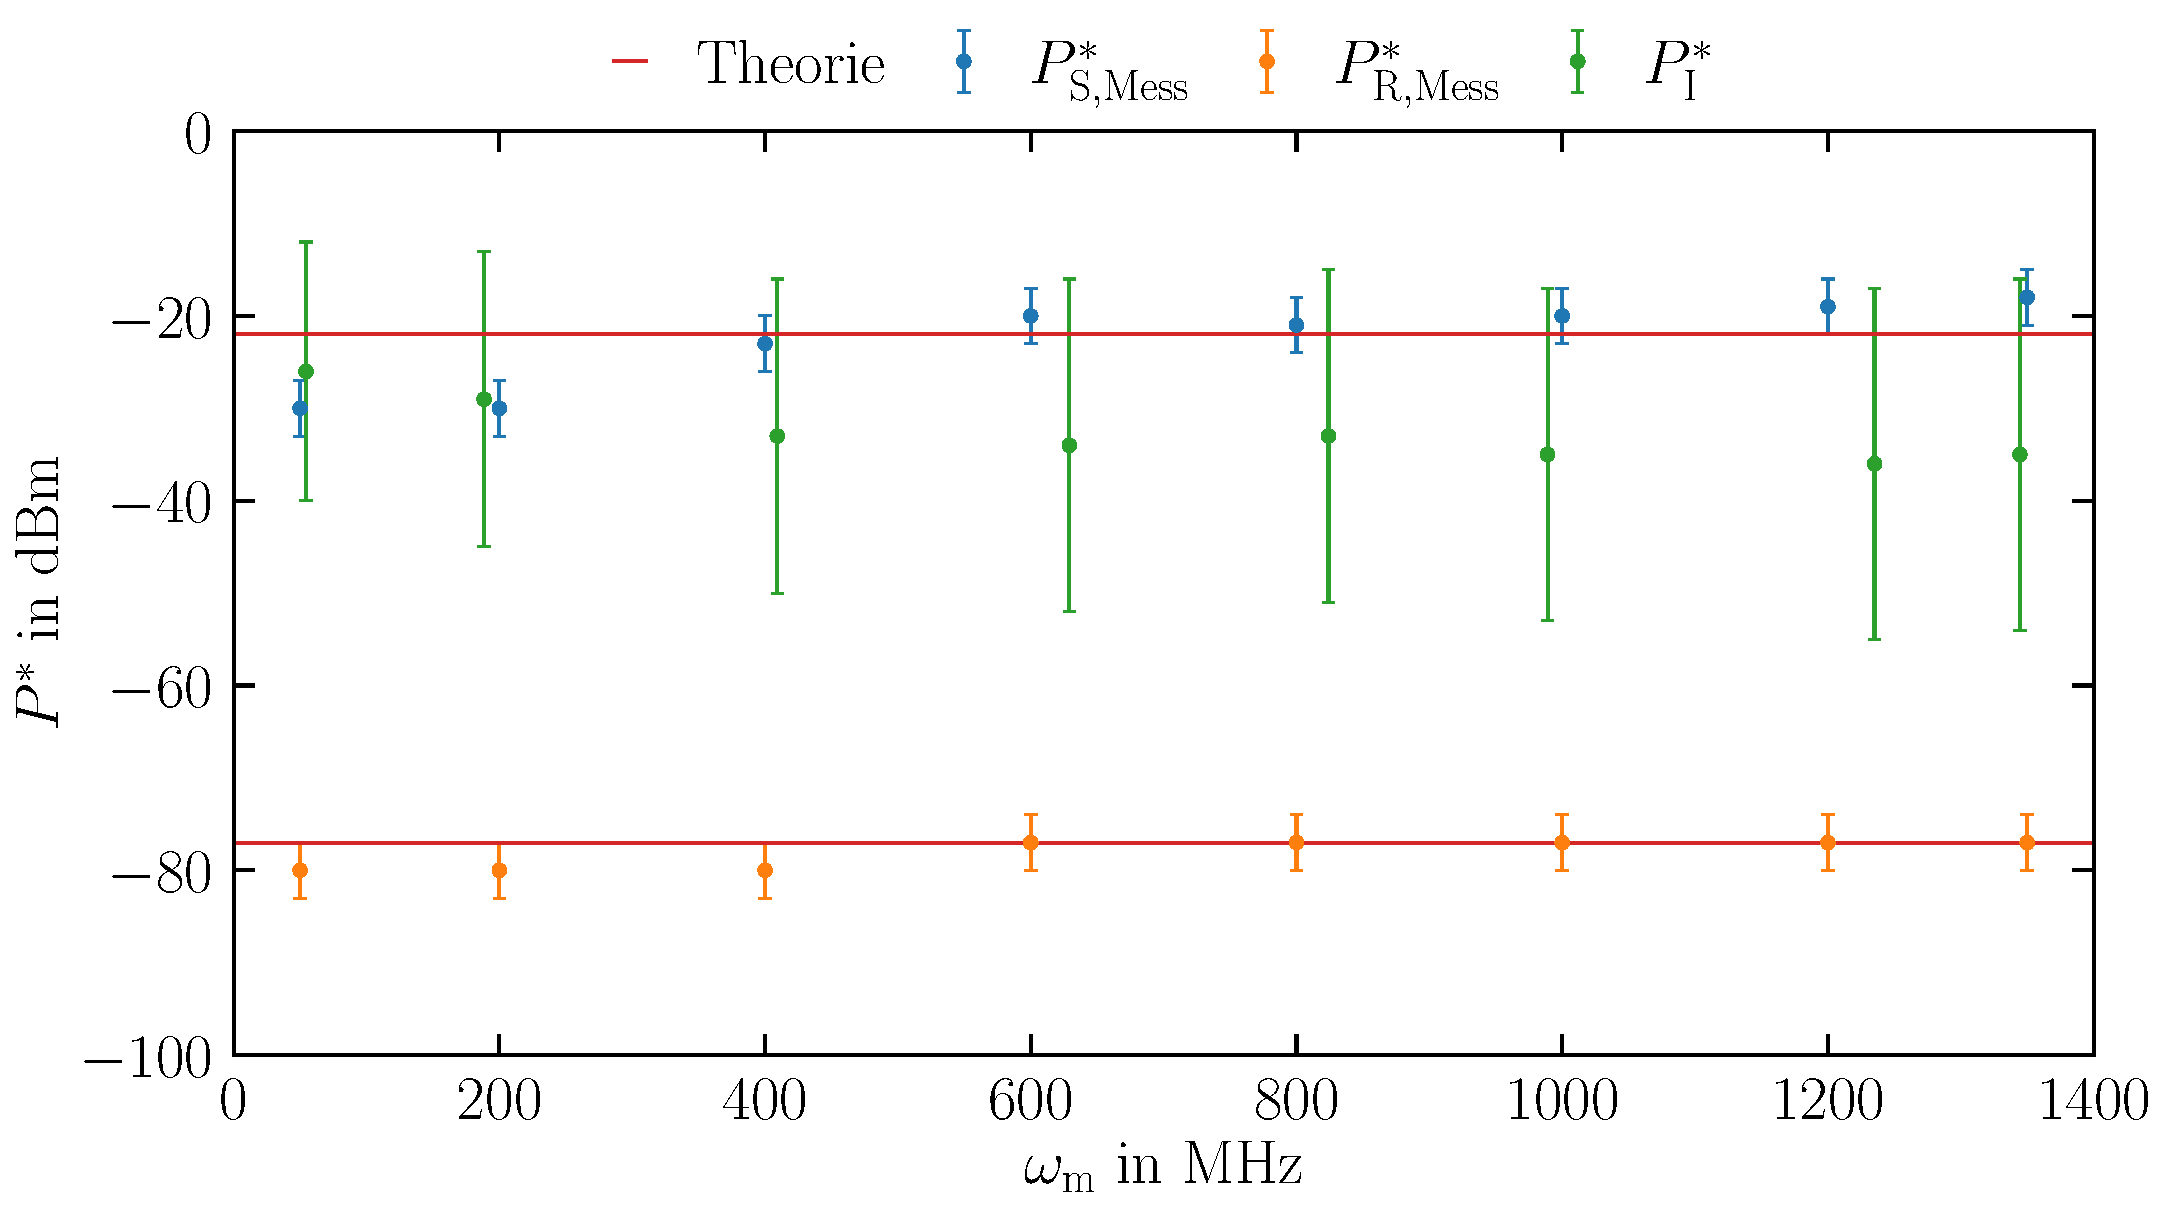
\includegraphics[scale=0.35]{Bilder/Auswertung/62/Signal-Rausch.pdf}
    \captionof{figure}{Vergleich zwischen Theorie und Praxis für gemessene Werte am Spekturmanalysator mit $P_\mathrm{R,Theo}$ = -77\,dBm und $P_\mathrm{S,Theo}$= -22\,dBm, sowie Vergleich zwischen $P_\mathrm{S,Mess}$ und $P_\mathrm{I}^*$}
    \label{fig:specAnalVergleich}
\end{center}

\subsection{Konversionsverluste}
\label{sub:konversionsverluste}

Nun werden die Werte des Spekturmanalysators, welches die Werte nach HF-Verstärker am R-Eingang des Mischer gemessen hat, mit den Werten nach dem NF-Verstärkers zu vergleichen. Dafür werden die Werte in Tabelle \ref{tab:verluste} durch den Faktor 31,5 geteilt (aus Skript entnommen) um die Spannung $U_\mathrm{I}$ vor den NF-Verstärkers zu erhalten. Danach wird angenommen, dass der Mischer ohne Konversionsverluste arbeitet, d.h. Eingang L und R haben keine Phasendifferenz, womit der Spannung am Ausgang I gleich der Spannung am Ausgang R ist, also $U_\mathrm{R} = U_\mathrm{I}$. Diese Spannung wird dann durch die Formel:
\begin{gather}
    P^*_\mathrm{I} = 10\cdot\log_{10}\left(\frac{U_\mathrm{I}^2}{2R}\cdot1000\right);~~[P^*] = 1\,\mathrm{dBm}
\end{gather}
in den gesuchten HF-Leistungswerte umgerechnet. \cite{anleitung} Beachte hierbei, dass der Widerstand $R=50\,\Omega$ \cite{anleitung} ist und der Faktor 1000 im Logarithmus die Umrechnung von 1\,W auf 1\,mW notwendig ist, um als Einheit für $P^*$ 1\,dBm zu erhalten. Der Vergleich zwischen $P^*_\mathrm{I}$ und $P_\mathrm{S,Mess}$ wurde graphisch in Abb. \ref{fig:specAnalVergleich} dargestellt. Eine skizzenhafte Darstellung des Schaltplans zur Übersicht ist in Abbildung \ref{fig:schaltschema} gegeben. 

\begin{center}
    \captionsetup{type=figure}
    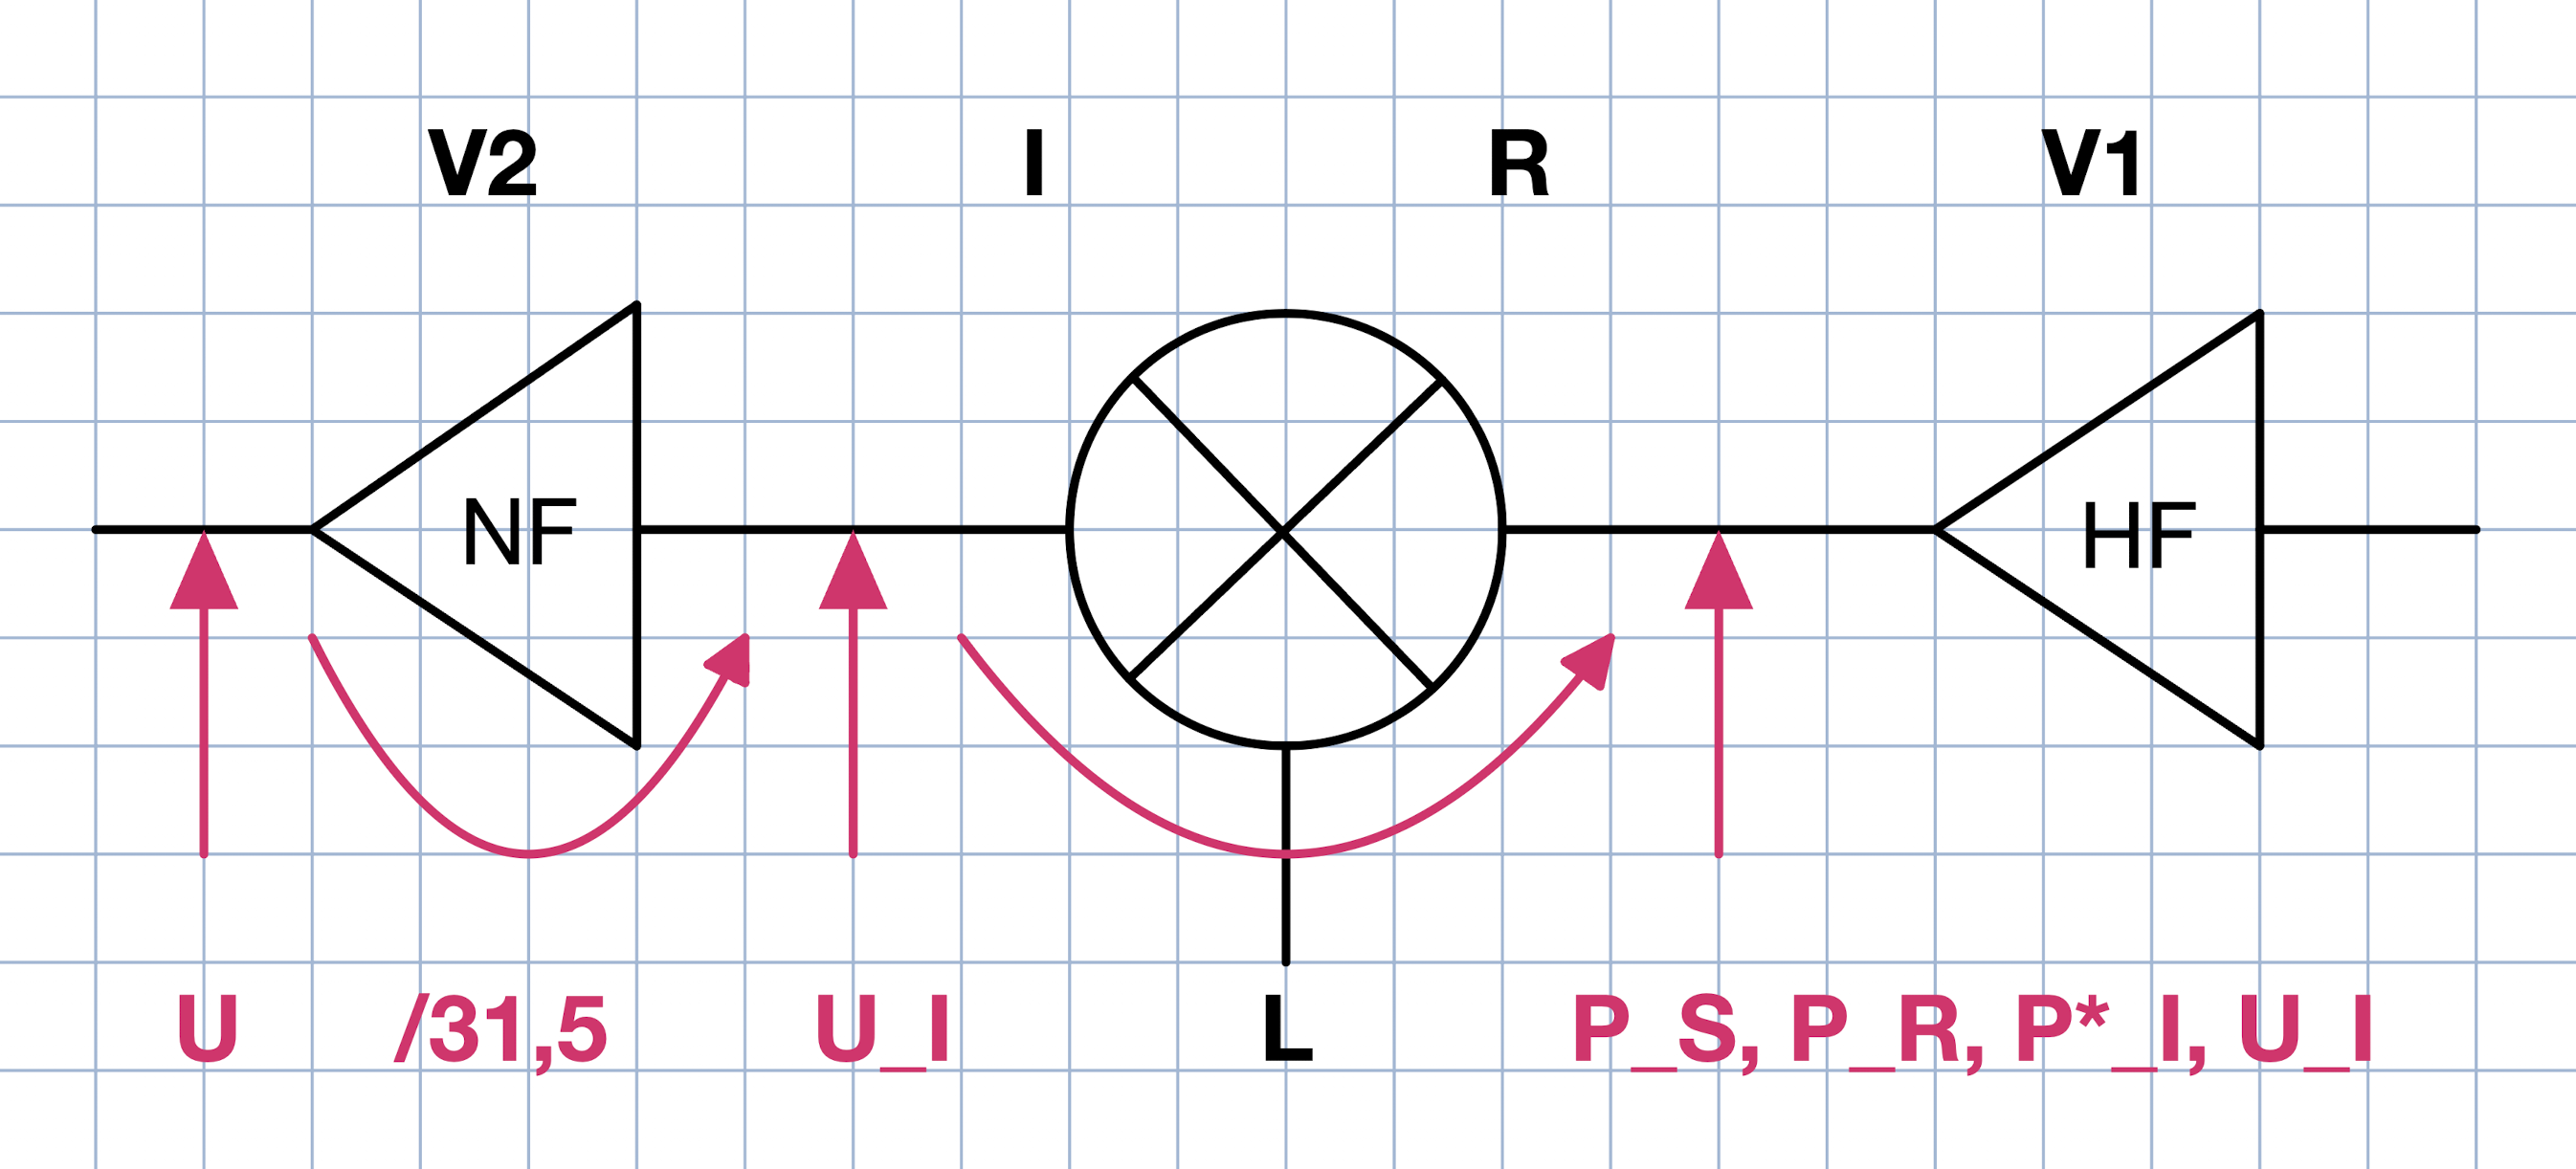
\includegraphics[scale=0.2]{Bilder/Schaltschema.png}
    \captionof{figure}{Skizze von der Anordnung der elektronischen Bauteile und Größen}
    \label{fig:schaltschema}
\end{center}

Um dann die konkreten Konversionsverluste zu ermitteln wird der Abstand zwischen $P^*_\mathrm{I}$ und $P_\mathrm{S,Mess}$ HF-Leistungswerte berechnet und der Mittelwert gebildet sowie die Standardabweichung. Dafür wird die Größe $v = |P^*_\mathrm{I} - P_\mathrm{S,Mess}|$ als Konversionsverlust eingeführt. Alles zusammen wird in Tabelle \ref{tab:konversionsverluste} dargestellt und die jeweiligen Fehler mit dem Fehlerfortpflanzungsgesetz berechnet. Die Berechnungen ergeben folgendes Ergebnis für den Konversionsverlust $v$:
\begin{gather}
    \boxed{v = (11 \pm 6)\,\mathrm{dBm}}~.
\end{gather}
Dies bedeutet, dass beim Mischen des Eingangsignals im Vergleich zum gemessenen Leistungspegel $P_\mathrm{S,Mess}$ ein Verlust von ungefähr die Hälfte des gemessenen Leistungspegels $P_\mathrm{S,Mess}$ auftritt. Weiterhin ist in Tabelle \ref{tab:konversionsverluste} zu erkennen, dass die mit steigender Modulationsfrequenz $\omega_\mathrm{m}$ der Konversionsverlust $v$ zunimmt.

\begin{center}
    \captionsetup{type=table}
    \begin{tabular}{r | c r | c c | r }
        $\omega_\mathrm{m}$/MHz & $U$/mV & $U_\mathrm{I}$/mV & $P_\mathrm{I}$/mW & $P^*_\mathrm{I}$/dBm & $v$/dBm\\ \hline
        54,5   & 208 $\pm$ 5 & 6.6  $\pm$ 0.2 &  436 $\pm$ 26 & -26 $\pm$ 14 &  4\\
        188,5  & 293 $\pm$ 5 & 9.3  $\pm$ 0.2 &  865 $\pm$ 37 & -29 $\pm$ 16 &  1\\
        409,2  & 421 $\pm$ 5 & 13.4 $\pm$ 0.2 & 1796 $\pm$ 54 & -33 $\pm$ 17 & 10\\
        629,1  & 511 $\pm$ 5 & 16.2 $\pm$ 0.2 & 2624 $\pm$ 65 & -34 $\pm$ 18 & 14\\
        824,1  & 452 $\pm$ 5 & 14.3 $\pm$ 0.2 & 2045 $\pm$ 57 & -33 $\pm$ 18 & 12\\
        989,0  & 533 $\pm$ 5 & 16.9 $\pm$ 0.2 & 2856 $\pm$ 68 & -35 $\pm$ 18 & 15\\
        1235,1 & 635 $\pm$ 5 & 20.2 $\pm$ 0.2 & 4080 $\pm$ 81 & -36 $\pm$ 19 & 17\\
        1344,5 & 572 $\pm$ 5 & 18.2 $\pm$ 0.2 & 3312 $\pm$ 73 & -35 $\pm$ 19 & 17\\
    \end{tabular}
    \captionof{table}{Berechnete Werte für Konversionsverluste}
    \label{tab:konversionsverluste}
\end{center}

\subsection{Effektive Quantenausbeute}
\label{sub:ausbeute}

Im nächsten Abschnitt wird die Quantenausbeute $\beta_\mathrm{D}$ berechnet. Dafür wird Gleichung (\ref{eq:leistungPhotosignal}) aus Kapitel \ref{sec:signalRausch} verwendet, welche hier nur nochmal aufgeführt und auf die Quantenausbeute $\beta_\mathrm{D}$ umgestellt wird:
\begin{gather}
    P_\mathrm{S,Mess} = \frac{1}{\sqrt{2}}\frac{\beta_\mathrm{D}}{2} P M \frac{\ln10}{2} \mathrm{OD}\\[0,5cm]
    \Leftrightarrow \beta_\mathrm{D} = \frac{4\sqrt{2}}{\ln10}\cdot\frac{P_\mathrm{S,Mess}}{P\cdot M}\cdot\frac{1}{\mathrm{OD}}~.
\end{gather}
Als HF-Leistungswerte $P_\mathrm{S,Mess}$ werden die gemessene Werte aus Kapitel \ref{sub:specAnal} verwendet. Die optische Dichte OD ist in Kapitel \ref{sub:opDichte} als OD = 0,09 $\pm$ 0,07 gegeben. Weiterhin ist der Modulationsindex $M$ zu jeder Modulationsfrequenz $\omega_\mathrm{m}$ in Kapitel \ref{sec:mindex} zu finden. Die Lichtleistung $P$ der Photodiode ist im Skript gegeben mit 0,135\,mW. Zuerst müssen die Leistungswerte $P_\mathrm{S,Mess}$ in mW umgerechnet werden, dafür wird der Verstärkungsfaktor von 55\,dB auf $P_\mathrm{S,Mess}$ addiert und dann mit der Formel:
\begin{gather}
    P^* = 10\log_{10}(P) \Leftrightarrow P = 10^{P^*/10}
\end{gather}
umgerechnet. \cite{anleitung} Dabei ist $P^*$ der Leistungspegel in dBm und $P$ der Leistungspegel in mW. Tabelle \ref{tab:ausbeute} fasst nochmal alle Werte an einer Stelle zusammen, sowie die errechneten Werte für die Quantenausbeute $\beta_\mathrm{D}$. Messfehler wurden mit dem Fehlerfortpflanzungsgesetz berechnet. In Tabelle \ref{tab:ausbeute} lässt sich bei niedrigen Modulationsfrequenzen eine hohe Quantenausbeute $\beta_\mathrm{D}$ erkennen, aber auch einen sehr großen Messfehler aufgrund der deutlich höheren Leistungswerte. Zudem muss einem klar sein, dass aufgrund der Umrechnung mit Basis 10 schon bei kleinen Ablesefehler große Unterschiede entstehen. Betrachtet man den Mittelwert der Quantenausbeute $\beta_\mathrm{D}$ erhält man als Ergebnis:
\begin{gather}
    \boxed{\beta_\mathrm{D} = 0,25 \pm 0,20}
\end{gather}
Eine herkömmliche Silizium-Photodiode erreicht heutzutage eine Quantenausbeute von 80\%, wobei schon mit sogenannten schwarzen Silizium eine Quantenausbeute von 130\% gelungen ist. \cite{siPD} Dies lässt darauf schließen, dass die gemessenen Werte noch in der Erwartung der Realität liegen.
\begin{center}
    \captionsetup{type=table}
    \begin{tabular}{r | c c | c c}
        $\omega_\mathrm{m}$/MHz & $P_\mathrm{S,Mess}$/dBm & $P_\mathrm{S,Mess}$/mW & $M$ & $\beta_\mathrm{D}$\\ \hline
        50   & -30 $\pm$ 3 & 0.00316 $\pm$ 0.00063 & 0,88 $\pm$ 0,02 & 0.73 $\pm$ 0.59 \\
        200  & -30 $\pm$ 3 & 0.00316 $\pm$ 0.00063 & 0,86 $\pm$ 0,02 & 0.74 $\pm$ 0.59 \\
        400  & -23 $\pm$ 3 & 0.00063 $\pm$ 0.00013 & 0,87 $\pm$ 0,02 & 0.15 $\pm$ 0.12 \\
        600  & -20 $\pm$ 3 & 0.00032 $\pm$ 0.00006 & 0,85 $\pm$ 0,02 & 0.08 $\pm$ 0.06 \\
        800  & -21 $\pm$ 3 & 0.00040 $\pm$ 0.00008 & 0,90 $\pm$ 0,02 & 0.09 $\pm$ 0.07 \\
        1000 & -20 $\pm$ 3 & 0.00032 $\pm$ 0.00006 & 0,91 $\pm$ 0,02 & 0.07 $\pm$ 0.06 \\
        1200 & -19 $\pm$ 3 & 0.00025 $\pm$ 0.00005 & 0,90 $\pm$ 0,02 & 0.06 $\pm$ 0.05 \\
        1350 & -18 $\pm$ 3 & 0.00020 $\pm$ 0.00004 & 0,91 $\pm$ 0,02 & 0.04 $\pm$ 0.03 \\
    \end{tabular}
    \captionof{table}{Berechnete Werte für Quantenausbeute}
    \label{tab:ausbeute}
\end{center}

\subsection{Minimale optische Dichte}
\label{sub:minopDichte}







